\textbf{เกี่ยวกับการเคลื่อนที่เป็นเส้นตรงในแนวดิ่ง}
\tcblower 
\begin{minipage}{0.6\linewidth}
ขณะวัตถุเคลื่อนที่ในแนวดิ่งวัตถุจะถูกแรงดึงดูดของโลกดูดเอาไว้  ทำให้เกิดความเร่งเนื่องจากแรงโน้มถ่วงในทิศพุ่งลงสู่พื้นโลก \hfill และมีขนาดประมาณ  \\ 9.8  เมตร/วินาที$^2$  ความเร่งนี้นิยมใช้สัญลักษณ์แทนด้วย  g
\end{minipage}\hfill
\begin{adjustbox}{valign=c} \begin{minipage}[t]{.35\linewidth}
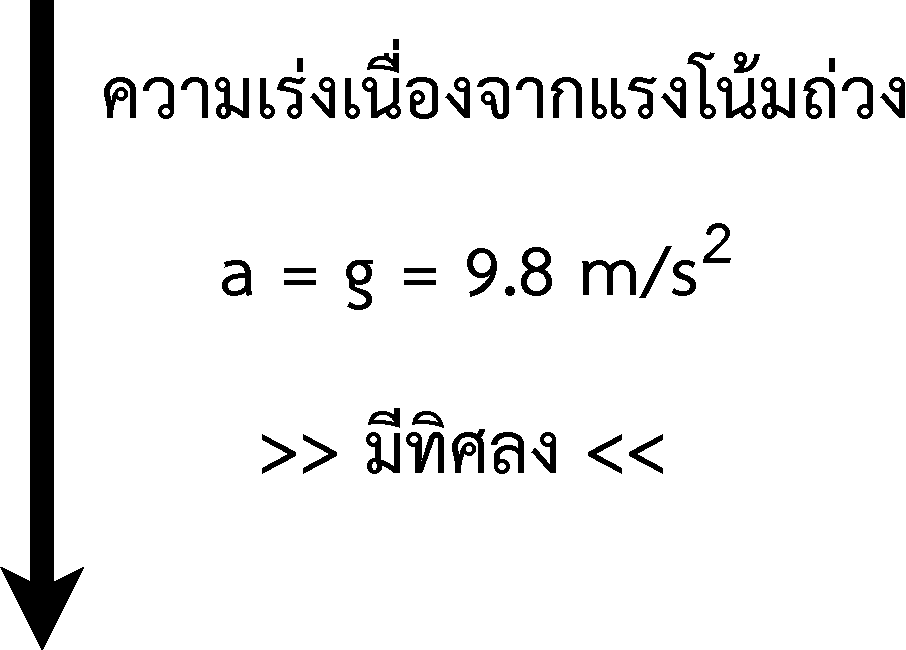
\includegraphics[width=\linewidth]{content-6.pdf}
\end{minipage}
\end{adjustbox}
